\documentclass[a4paper,12pt]{report}

\usepackage{alltt, fancyvrb, url}
\usepackage{graphicx}
\usepackage[utf8]{inputenc}
\usepackage{float}
\usepackage{xcolor}
\usepackage{hyperref}

% Questo commentalo se vuoi scrivere in inglese.
\usepackage[italian]{babel}

\usepackage[italian]{cleveref}

%---------------
\newcommand{\imgpath}{img/png}
%---------------

%\title{Meta-relazione per\\``Programmazione ad Oggetti''}
\title{Javamant \\ Relazione per il progetto del corso OOP}

\author{
	Filippo Gaggi
	\\ Andrea La Tosa
	\\ Emir Wanes Aouioua}
\date{\today}


\begin{document}

\maketitle

\tableofcontents

\chapter{Analisi}

\section{Descrizione e requisiti}

Il progetto ha come scopo la realizzazione di una trasposizione digitale del gioco
da tavolo DIAMANT.
Il gioco simula l'esplorazione di grotte, in cui i giocatori
(dai 3 agli 8) cercano di accumulare il maggior numero possibile di gemme.
Alla fine di una serie di round il vincitore sarà colui che riuscirà
a raccogliere il maggior numero di gemme. L'esplorazione di una grotta è rappresentata da un round.
%
Il percorso di esplorazione di una grotta rappresenta le carte pescate da un mazzo durante il round,
le quali possono essere di tre tipi:
\begin{itemize}
	\item \textbf{Carte tesoro}, 15 nel mazzo standard. Rappresentano una quantità di gemme da dividere tra i giocatori in esplorazione nella grotta.
			La divisione delle gemme delle carte tesoro è equa tra i giocatori:
			il resto della divisione rimane all'interno del percorso di esplorazione.
	\item \textbf{Carte trappola}, 15 nel mazzo standard. Rappresentano ostacoli per i giocatori. Pescare due carte trappola
	identiche fa terminare il round forzatamente e fa perdere tutte le gemme guadagnate nell'esplorazione
	della grotta ai giocatori che non hanno abbandonato quest'ultima.
	\item \textbf{Carte reliquia}, 5 nel mazzo standard. Le reliquie hanno un valore in gemme e, a differenza delle carte tesoro,
		il valore in gemme di quest'ultime non viene distribuito tra i giocatori: le gemme relative alle
		carte reliquia vengono assegnate ad un solo giocatore, nel caso in cui esso decida di abbandonare
		l'esplorazione della grotta da solo.
\end{itemize}

Ogni giocatore possiede una sacca per raccogliere le gemme trovate durante l'esplorazione della grotta
ed un forziere dove conservare le gemme alla fine dell'esplorazione di quest'ultima.
\\
L'esplorazione di una grotta si svolge in turni. Ogni turno
è suddiviso in due fasi:
\begin{itemize}
	\item \textbf{Fase di estrazione}: il giocatore del turno pesca una carta dal mazzo, la aggiunge al percorso di esplorazione
		e distribuisce eventuali gemme tra i giocatori presenti nella grotta; in caso di trappola doppia
		il round termina. 
	\item \textbf{Fase di decisione}: tutti i giocatori all'interno della grotta decidono se continuare
		ad esplorare quest'ultima o se uscire. I giocatori uscenti dividono le gemme rimaste nel percorso di esplorazione
		e le depositano, assieme alla propria sacca, all'interno del rispettivo forziere.
\end{itemize}

Il gioco si fonda su un fattore di rischio legato alla decisione sul proseguimento dell'esplorazione:
\begin{itemize}
	\item \textbf{Continuare l'esplorazione} comporta possibilmente un maggior numero di gemme guadagnato
	ma aumenta il rischio che due trappole identiche vengano pescate: in tal caso tutte le gemme
	dei giocatori rimasti in esplorazione della grotta non vengono aggiunte ai rispettivi forzieri.
	\item \textbf{Abbandonare l'esplorazione} preclude il giocatore dal trovare altre gemme ma gli permette
	di mettere al sicuro le gemme della sua sacca all'interno del proprio forziere, oltre a quelle delle
	carte reliquia se è abbastanza fortunato da abbandonare il round da solo durante il turno.
\end{itemize}
La trasposizione digitale del gioco prevede inoltre la possibilità di applicare
degli effetti speciali al round che modificano il modo in cui l'esplorazione di una grotta termina
(nella versione standard attraverso due carte trappola identiche pescate) e delle variazioni
al numero di gemme guadagnate dai giocatori.

\subsubsection{Requisiti funzionali}
\begin{itemize}
	\item Il sistema deve gestire un mazzo di 35 carte divise in tre categorie (tesoro, trappola, reliquia).
	\item L'applicazione deve supportare partite da 3 ad 8 giocatori con la possibilità di giocatori comandati dal software.
	\item I turni dovranno essere composti da due fasi in sequenza: l'estrazione della carta
	e la decisione da parte di tutti i giocatori nella grotta sul continuare l'esplorazione. 
	\item Dovrà essere possibile estrarre
	una carta e la sua visualizzazione nel percorso di esplorazione.
	\item L'applicazione deve calcolare la divisione equa delle gemme tra i giocatori attivi,
	tenendo in considerazione le gemme già rimaste sul percorso ed eventuali modificatori
	applicati a quest'ultime.
	\item La partita deve terminare automaticamente non appena due carte trappola identiche
	vengono pescate durante un round, oppure se l'effetto speciale del round ne decreta il termine.
	\item Il sistema deve tracciare le gemme di ogni giocatore, sia nella sacca che nel forziere;
	il sistema deve stilare una classifica dei giocatori al termine di tutti i round
	che sia ordinata in base al numero di gemme nei forzieri.
	\item L'applicazione deve gestire l'assegnazione delle relique nel caso un solo giocatore
	esca dalla partita. 
\end{itemize}

\subsubsection{Requisiti non funzionali}
\begin{itemize}
	\item L'architettura software deve essere progettata in modo modulare
	per permettere una facile estendibilità delle carte e degli effetti del round.
	\item L'interfaccia grafica dovrà essere chiara ed intuitiva, permettere la visualizzazione dei turni, delle carte pescate e dei punteggi.
	\item I bot devono utilizzare strategie logiche in base allo stato della partita.
	\item Il sistema deve dare la possibilità di configurare la partita: decidere il numero di round,
	gli effetti speciali, il deck usato e la presenza o meno di bot.
\end{itemize}

\section{Modello del Dominio}

L'applicazione Javamant modella l'esplorazione di grotte,
ognuna rappresentata da un round. Ogni partita coinvolge
dei giocatori, che possono essere controllati da umani o
dal software. Ogni round utilizza un mazzo di carte che
progressivamente formeranno il percorso di esplorazione della grotta.
Le carte pescate dal mazzo si dividono in più tipi: le carte tesoro forniscono
gemme da distribuire equamente tra i giocatori, le carte trappola
rappresentano pericoli che possono, se l'effetto del round lo permette, terminare il round e le carte
reliquia danno gemme aggiuntive se un solo giocatore abbandona l'esplorazione
alla fine di un turno.
Un round si divide in turni successivi, ognuno composto da due fasi.
Nella fase di estrazione il giocatore del turno pesca la carta che
viene aggiunta al percorso dell'esplorazione. Nella fase di decisione
i giocatori che esplorano la grotta scelgono se continuare l'esplorazione.
Tutti i giocatori hanno una sacca temporanea per raccogliere le gemme durante un
round ed un forziere per mantenere le proprie gemme tra un round e l'altro.
Ad ogni round viene associato un effetto speciale che ne determina
la condizione di fine e un eventuale modificatore applicato alle gemme.



\subsection*{Elementi positivi}
\begin{itemize}
	\item Si modella il dominio in forma di UML\@.
	\item Viene descritto accuratamente il modello del dominio.
	\item Il modello cattura le entità di dominio, le loro caratteristiche principali,
	\item e le relazioni che intercorrono fra di loro.
\end{itemize}

\subsection*{Elementi negativi}
\begin{itemize}
	\item Manca una descrizione a parole del modello del dominio.
	\item Manca una descrizione UML delle entità del dominio e delle relazioni che intercorrono fra loro.
	\item Vengono presentati elementi di design, o peggio, implementativi.
	\item Viene mostrato uno schema UML che include elementi implementativi o non utili alla descrizione del dominio,
	ma volti alla soluzione (non devono vedersi, ad esempio, campi o metodi privati).
\end{itemize}

% !!!!!!!!!!!!!!!!!!!!!!!!!!!!!!!!!!!!!!!!!!!!!!!!
% QUA C'E' DA METTERE L'UML ASTRATTISSIMO DEL DOMINIO.

\subsection*{Esempio}
GLaDOS dovrà essere in grado di accedere ad un'insieme di camere di test.
%
Tale insieme di camere prende il nome di percorso.
%
Ciascuna camera è composta di challenge successivi.
%
GLaDOS è responsabile di associare a ciascun challenge un insieme di consigli (suggestions) destinati all'utente (subject), dipendenti da possibili eventi.
%
GLaDOS dovrà poter comunicare coi locali cucina per approntare le torte.
%
Le torte potranno essere dolci, oppure semplici promesse di dolci che verranno disattese.
%
Gli elementi costitutivi il problema sono sintetizzati in \Cref{img:analysis}.

Data la complessità di elaborare consigli via AI senza intervento umano, la prima versione del software fornita prevederà una serie di consigli forniti dall'utente.
%
Il requisito non funzionale riguardante il consumo energetico richiederà studi specifici sulle performance di GLaDOS che non potranno essere effettuati all'interno del monte ore previsto: tale feature sarà oggetto di futuri lavori.

\begin{figure}[H]
	\centering{}
	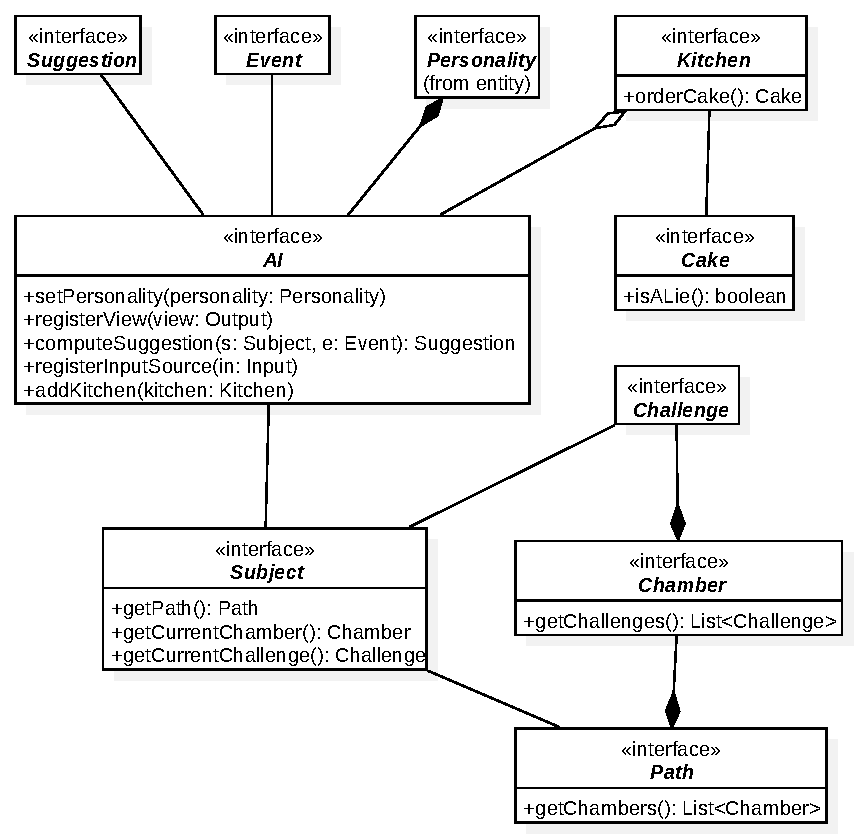
\includegraphics{img/analysis.pdf}
	\caption{Schema UML dell'analisi del problema, con rappresentate le entità principali ed i rapporti fra loro}
	\label{img:analysis}
\end{figure}

\chapter{Design}

\section{Architettura}

L'achitettura di Javamant adotta il pattern architettura Model View Controller (MVC) per
dare una separazione ai ruoli dei componenti principali, minimizzando le dipendenze.
In particolare:

\begin{itemize}
	\item \textbf{Model}: definito dall'interfaccia \textit{Game}; rappresenta il punto di accesso
	al dominio dell'applicazione.
	\item \textbf{View}: viene definita dalle interfacce \textit{Window} e \textit{Page} che
	rappresentano la finestra principale di visualizzazione e le singole pagine che possono
	essere rappresentate su di essa.
	\item \textbf{Controller}: definita da \textit{MainController}, il quale avvia l'applicazione,
	\textit{PageController} che definisce l'interazione su una pagina specifica e
	\textit{GameAwarePageController}, simile a PageController ma con accesso
	ad informazioni sul model (Game). I controller per le pagine gestiscono la navigazione
	tra queste ultime tramite \textit{PageNavigator}.
\end{itemize}

Le interazioni principali di questa architettura sono:
\begin{itemize}
	\item MainController gestisce tutte le dipendenze
	tra model, view e controller. Inizializza la Window,
	il PageNavigator, le varie Page e rispettivi PageController.
	\item GameAwarePageController estende PageController; interagisce con
	Game per recuperare informazioni sullo stato della partita.
	\item Ogni PageController è associato a un'unica Page e
	utilizza il PageNavigator per cambiare visualizzazione.
	\item Window ha il compito di essere un contenitore per Page e si
	occupa di mostrarle all'utente.
	\item PageNavigator gestisce la transizione
	da una pagina all'altra.
\end{itemize}

L'architettura è stata progettata in modo da poter sostituire
in modo semplice la view: per poter sostituire l'intera componente
grafica è sufficiente dare nuove implementazioni di \textit{Window}
e \textit{Page}, infatti i controller dipendono unicamente
da queste interfacce ed il model non mantiene alcun riferimento
ad elementi grafici.

Una versione schematizzata dell'architettura adoperata ~\ref{img:arch}:

\begin{figure}[H]   % H maiuscola
\centering
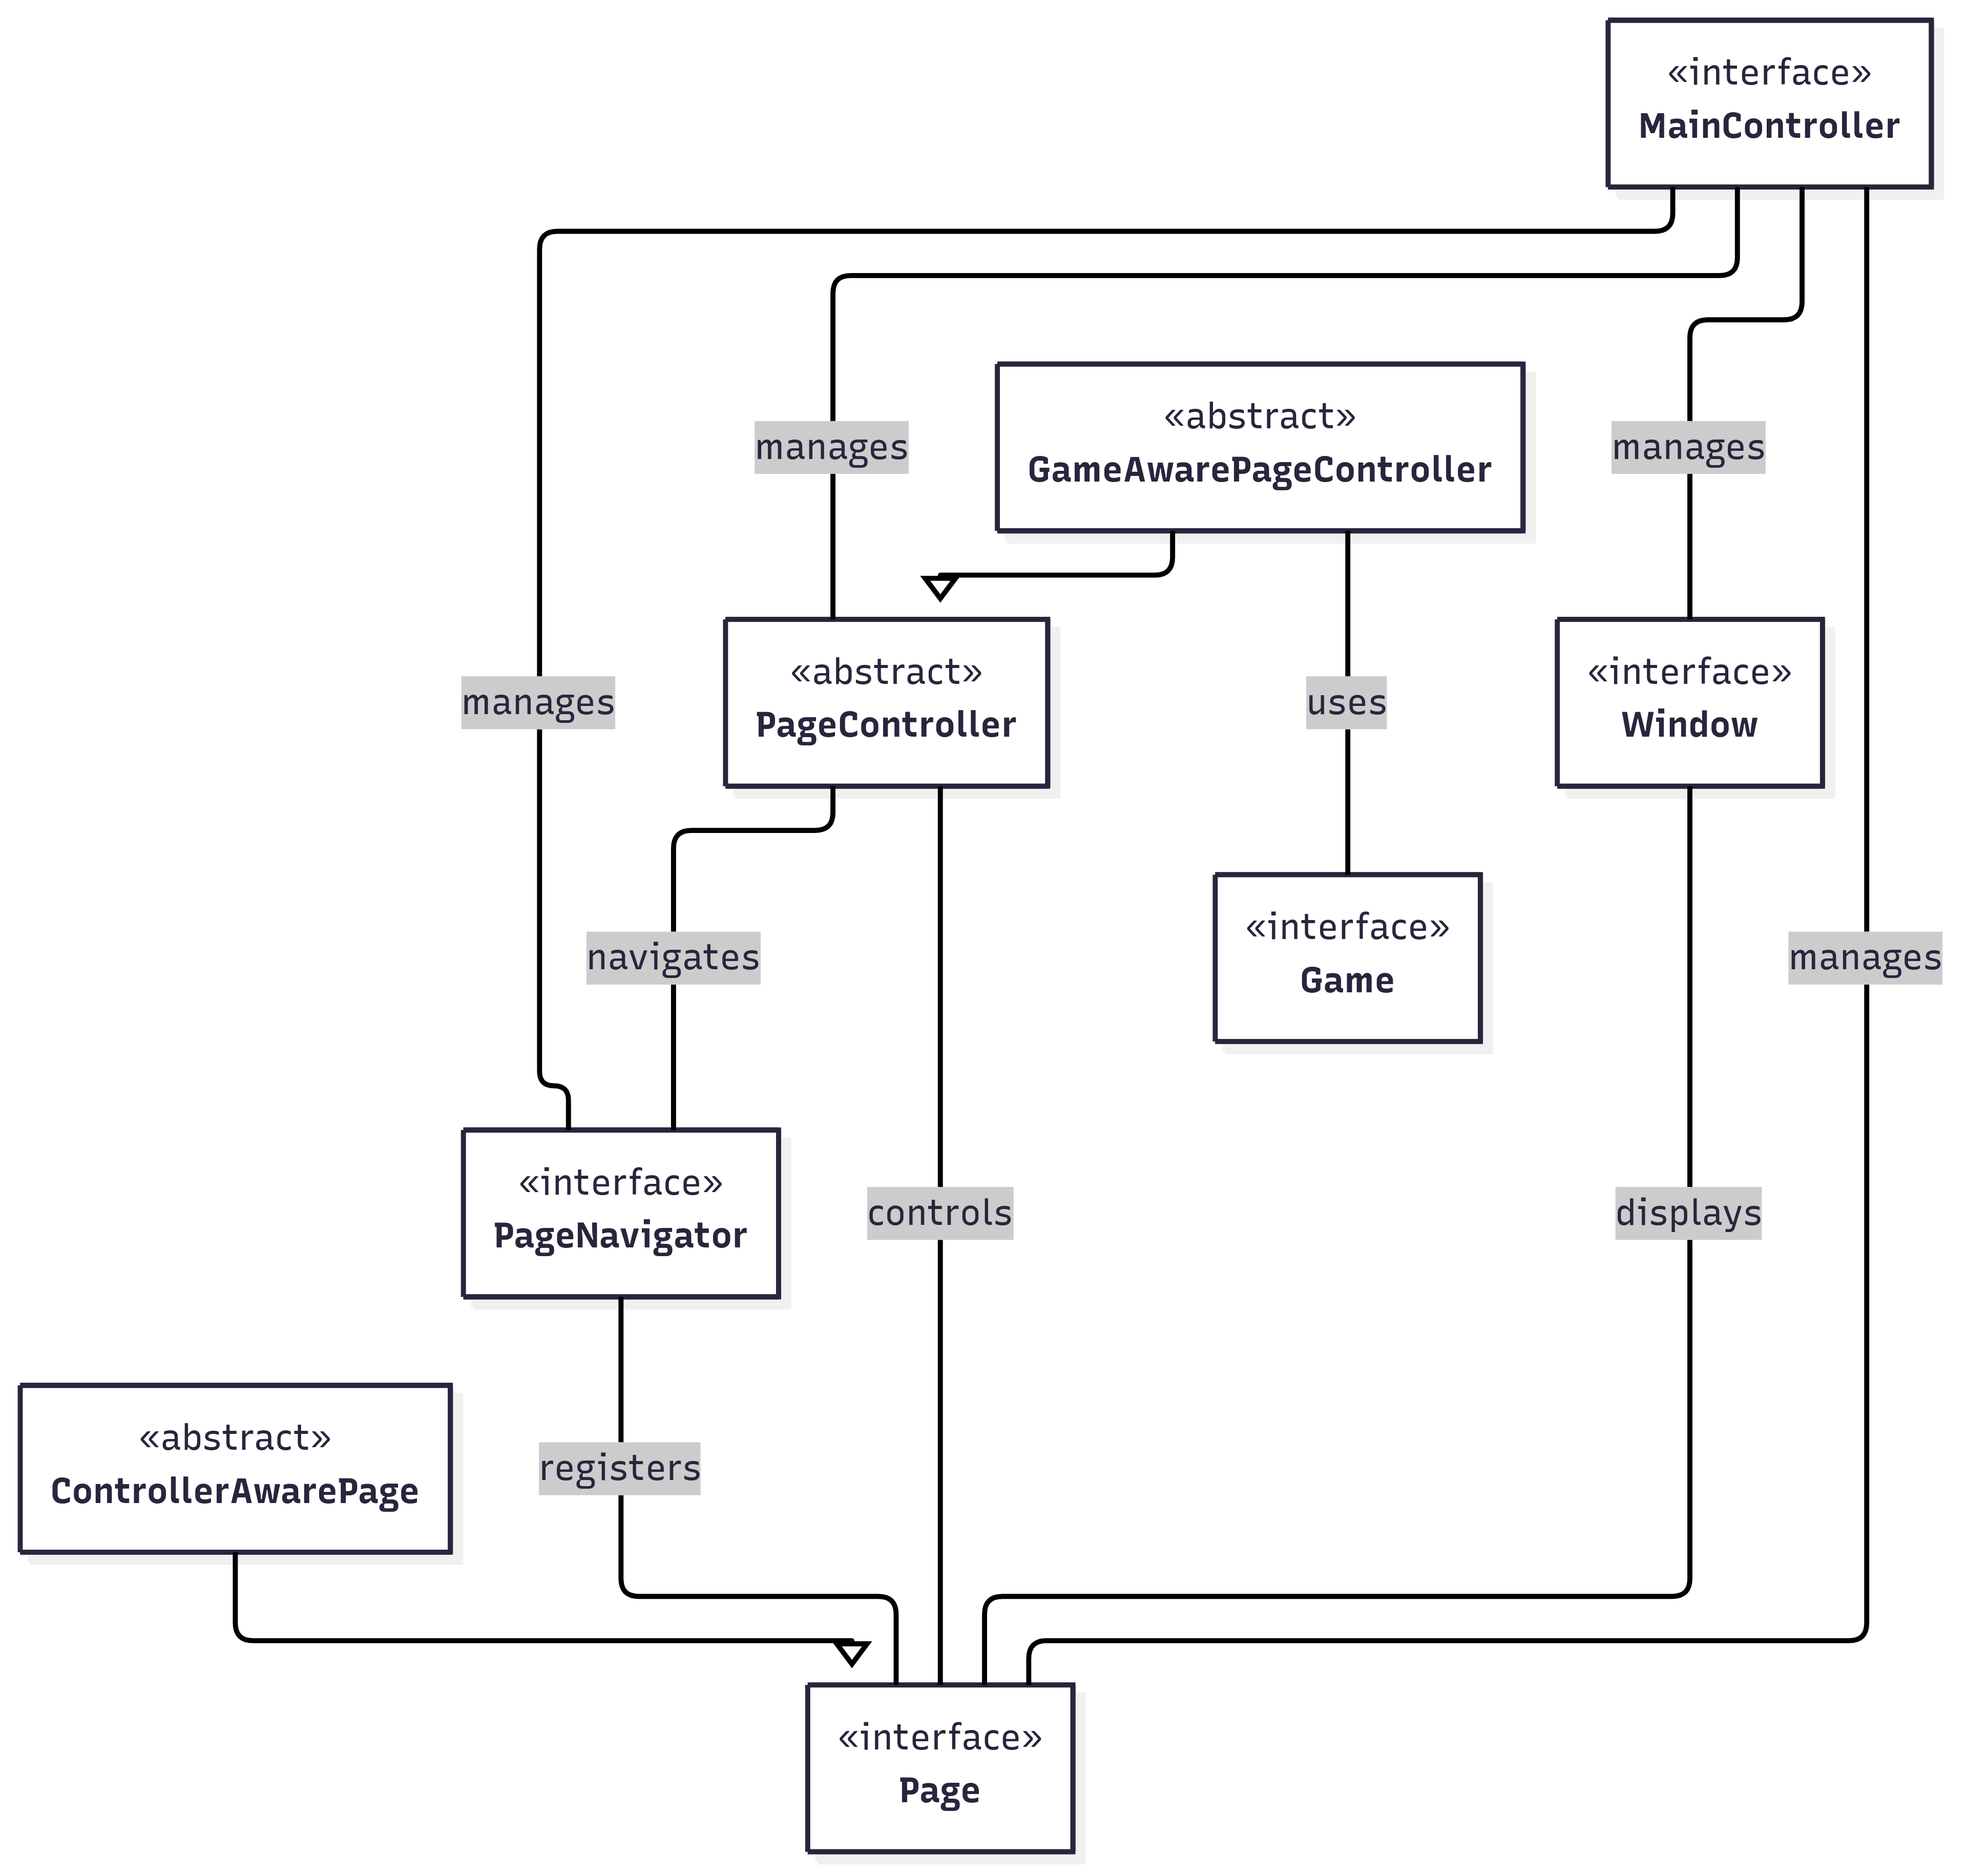
\includegraphics[width=\textwidth]{img/architecture}
\caption{Schema UML architetturale di Javamant.}
\label{img:arch}
\end{figure}


\section{Design dettagliato}

%------
\subsection{Andrea La Tosa}
\subsubsection{Refactoring classe DeckImpl:}

\paragraph{Problema:}

Durante lo sviluppo del progetto la classe DeckImpl (responsabile della gestione del mazzo di carte) stava mostrando i seguenti problemi architetturali:
\begin{itemize}
	\item era diventata una classe molto grande con molti metodi, difficile da manutenere ed estendere,
	\item  violava SRP(single responsibility principle),
	\item  era diventata una vera e propria God class accentrando dentro di sè troppe responsabilità.
\end{itemize}
%
DeckImpl aveva una classe annidata che aveva lo scopo di:
\begin{itemize}
	\item  calcolare le statistiche del mazzo(es. il numero di carte trappola, il numero totale di carte nel mazzo etc..) 
	restituendole alla classe contenitore che a sua volta le avrebbe restituite verso l'esterno 
	(logica poco intuitiva e ridondante),
	\item  creare i vari tipi di mazzo (standard e special),
	\item  includere i metodi per aggiungere le carte al mazzo.
\end{itemize}
%
Questa implementazione risultava quindi confusionaria e difficilmente manutenibile.

\paragraph{Refactoring effettuato:}

Per risolvere queste problematiche è stato effettuato un refactoring strutturale che ha portato la divisione della classe originaria 
in classi piu' semplici e con responsabiltà singole e ben definite adottando tre noti design pattern: Iterator, Builder e Factory.
Il refactoring ha portato alla definizione delle seguenti classi:
\begin{itemize}
	\item  DeckImpl: gestisce la logica del mazzo come le statistiche, il mescolamento e l'estrazione delle carte.
	Per quest'ultima funzionalità l'interfaccia della classe estende Iterator$<$Card$>$.
	\item  DeckBuilderImpl: applica il pattern Builder per aggiungere al mazzo i vari tipi di carte e infine,medinate il metodo build(), creare un oggetto Deck.
	\item  DeckFactoryImpl: applica il pattern Factory per la creazione di mazzi predefiniti (es. mazzo standard) sfruttando i metodi forniti da DeckBuilderImpl.
\end{itemize}

\paragraph{Benefici ottenuti dopo il refactoring:}

\begin{itemize}
	\item  manutenibilità: ogni classe ha una responsabilità piu' piccola e ben definita.
	\item  estendibilità: è molto piu' semplice aggiungere nuove funzionalità e configurazioni di mazzi.
	\item  testing: i test sono piu' semplici da effettuare non avendo piu' una God class.
\end{itemize}
%
\paragraph{Problematiche ottenute dopo il refactoring:}

\begin{itemize}
	\item  piu' interfacce e classi da gestire
	\item  la comprensione del codice potrebbe risultare inizialmente piu' complessa.
\end{itemize}

\begin{figure}[H]
	\centering
	
\includegraphics[height=0.9\textheight]{\imgpath/UML_Deck2.png}
	\caption{Diagramma UML dopo il refactoring della classe DeckImpl con l'utilizzo dei pattern Iterator, Builder e Factory}
	\label{fig:uml_deck_refactoring}
\end{figure}


\subsubsection{GERARCHIA DELLE CARTE:}

\paragraph{Problema:}

il gioco, come definito nella fase di analisi, prevede l'utilizzo di 4 tipologie di carte:
\begin{itemize}
	\item \textbf{Trappola:}
	non hanno valore in gemme.
	Vengono utilizzate per alcune condizioni di fine round.

	\item \textbf{Tesoro:}
	hanno un valore associato in gemme.

	\item \textbf{Reliquia:}
	hanno un valore associato in gemme estratto da una sequenza di possibili valori.
	
	\item \textbf{Speciale} (non ancora implementate):
	sono state pensate per aggiungere effetti particolari e dinamicità al gioco come ad esempio far perdere delle gemme dalla sacca di un giocatore.
	Possono avere o meno un valore in gemme.
\end{itemize}
Il design di progettazione doveva tener conto:
\begin{itemize}
	\item delle 3 tipologie di carte effettivamente implementate,

	\item della possibilità di estendere il gioco con le carte speciali.
\end{itemize}
La soluzione iniziale non permetteva nè di modellare in modo efficace la differenza tra carta tesoro e reliquia nè una facile estensione per le carte speciali.

\subsection*{Soluzione iniziale:}

Il  primo approccio prevedeva una gerarchia con la seguente struttura:
\begin{itemize}
	\item Card:
	la classe principale che definisce i comportamenti comuni a tutte le carte.
	\item TreasureCard, RelicCard, TrapCard:
	le classi che estendono Card e definiscono i comportamenti specifici delle rispettive carte.
\end{itemize}
%
Tuttavia, in questo tipo di gerarchia era evidente la duplicazione della logica tra il comportamento delle carte reliquia e reperto.
L'unica differenza era il come veniva generato il numero di gemme da associare alla carta:
internamente per le carte reliquia e richiesto in input per le carte tesoro.
\\\\
Questa struttura non solo violava il principio DRY(Don't Repeat Yourself) ma rendeva la gerarchia poco estendibile.

\paragraph{Refactoring effettuato:}

Per risolvere il problema è stata aggiunta la classe intermedia CardWithGem.
Questa descrive il comportamento generico delle carte (estendendo Card) ma aggiunge la logica delle gemme.
Le classi RelicCard e TreasureCard estendono ora CardWithGem evitando la duplicazione di logica e codice.

\begin{figure}[H]
	\centering
	
\includegraphics[width=0.8\textwidth]{\imgpath/UML_Card.png}
	\caption{Diagramma UML della gerarchia delle carte dopo l'introduzione della classe intermedia CardWithGem}
	\label{fig:uml_card_hierarchy}
\end{figure}

\noindent Questo refactoring ha anche anticipato l'aggiunta delle carte speciali in quanto:
\begin{itemize}
	\item se hanno delle gemme potranno estendere CardWithGem
	\item se non hanno delle gemme potranno estendere Card
\end{itemize}

\chapter{Sviluppo}
\section{Testing automatizzato}

%-----------
Il testing automatizzato è stato effettuato con Junit, di seguito i vari test divisi per sezioni:
\begin{itemize}
 \item Card:
    \begin{itemize}
    \item DeckTest: i test sono stati effettuati sulla configurazione standard del deck, comprendono la corretta composizione del mazzo e l'estrazione delle carte.
	\item TrapCardTest: testing riguardante il comportamento comune delle carte.
	\item RelicCardTest: oltre ai test sui metodi comuni delle carte è stato verificato anche il riscatto, lo stato relativo e i valori di gemme possibili.
	\item TreasureCardTest: oltre ai test sui metodi comuni delle carte sono stati verificati i valori di gemme ammessi.
    \end{itemize}
 \item Round:
    \begin{itemize}
    \item EndConditionFactoryImplTest:
    \item GemModifierFactoryImplTest:
    \item RoundImplTest:
    \item RoundPlayersManagerImplTest:
    \item RoundStateImplTest:
    \item TurnImplTest:
    \item FullGameTest:
    \end{itemize}
 \item Player:
    \begin{itemize}
    \item LogicCpuTest: Testing riguardante la correttezza di comportamento di LogicCpuImpl nelle 3 difficoltà.
    \item PlayerInRoundTest: Testing riguardante la correttezza dei metodi di PlayerInRound.
    \item PlayerCpuTest: Testing riguardante la correttezza dei metodi di PlayerCpu.
    \end{itemize}
 \item Settings:
    \begin{itemize}
    \item GameSettingsTest: Testing riguardante la correttezza di comportamento dei controlli di GameSettingsImpl.
    \end{itemize}
 \item Leaderboard:
    \begin{itemize}
    \item LeaderboardTest: Testing riguardante la correttezza dei metodi di LeaderboardImpl.
    \end{itemize}
\end{itemize}

%----------

\section{Note di sviluppo}

\subsection{Andrea La Tosa}

\subsubsection{Utilizzo di generici:} \url{https://github.com/Wanes01/OOP24-jvmt/blob/bbeaba836d375717ec403006b1f065be8725656e/src/main/java/jvmt/view/page/utility/ComboboxWithLabel.java#L91C1-L96C6}

\subsubsection{Utilizzo di stream e lambda:} \url{https://github.com/Wanes01/OOP24-jvmt/blob/ccdbae592c490476d3226350cbdbbeb99e32a596/src/main/java/jvmt/view/page/impl/SwingSettingsPage.java#L313C9-L318C10}

\subsubsection{Utilizzo della dipendenza esterna MigLayout:}
Utilizzato in vari punti, un esempio: \url{https://github.com/Wanes01/OOP24-jvmt/blob/ccdbae592c490476d3226350cbdbbeb99e32a596/src/main/java/jvmt/view/page/impl/SwingSettingsPage.java#L189C17-L192C50}

\subsubsection{Utilizzo di consumer:} \url{https://github.com/Wanes01/OOP24-jvmt/blob/ccdbae592c490476d3226350cbdbbeb99e32a596/src/main/java/jvmt/controller/impl/SettingsControllerImpl.java#L93C1-L93C49}
%------------------



\chapter{Commenti finali}

\section{Autovalutazione e lavori futuri}

\subsection{Andrea La Tosa}
Ho svolto la mia parte di progetto al meglio delle mie capacità e ritengo di aver dato un valido contributo al gruppo.
Il progetto è stato svolto in un ambiente sereno e tranquillo il che ha reso molto facile scambiarsi idee e punti di vista, senza i quali avrei prodotto codice meno leggibile e manutenibile.
Sono molto contento del codice che ho prodotto anche se devo ammettere che ho percepito molto la mia inesperienza in certi argomenti, primo fra tutti GitHub. 


\appendix
\chapter{Guida utente}

\end{document}
